\chapter{Tilpasning af skalaer}
\label{TestAfSkalaTilpasningAfSkalaer}
%
%Diskuter hvordan vi vælger at tilpasse skalaerne efter skalatype - altså skal de alle sammen være ens og skal alle skala spørgsmål være ens
De udviklede skaler i \fullref{ParametreDatabehandlingSkalaer} bør tilpasses før de præsenteres i en test, så skalaerne er konsistente og derved letter at besvarer for testpersonerne. \blankline
%
Ved tilpasningen er der fokus på at anvende samme formulering og ordvalg i skalaerne.

(Her kommer en beskrivelse af hvordan vi tilpasser de 24 skalaer og labels, så de er nemme at besvarer for testpersonerne - Det er her vi bl.a. tager stilling til om vi skal have både bipolær og unipolær, eller kun én af dem.) 

\section{Rækkefølgen på skalaerne}
(Her skriver vi om de to skalaspørgsmål der kommer til sidst, og at resten randomiseres, så det blandes.)


Årsagen til at en skala omformuleres i forhold til labels, spørgsmål og skala type er for at undgå bias (eller lægge ord i munden på folk) eller fordi spørgsmål og label decideret ikke passer sammen i forhold til at fuldende en sætning. Derefter vurderes det hvor den specifikke skala passer hen - så der kan dannes "grupper" af konsistente skalaer.\blankline 
%
SQ: Hvordan synes du skærmen reagerede? Vi vælger ikke at komme label på midt punktet da vi tænker at det er intuitivt at midten mellem dårligt og godt er "halvdelen/neutralt". Det kommer som det første skala spørgsmål, hver gang. Derudover tilføjer vi: på robotten\blankline
%
SQ: Hvor meget kendskab har du til teknologi? Vi sletter robotter, vi vælger teknologi fordi det dækker over mere. \blankline
%
SQ: Jeg kan godt lide at blive betjent af robotten får nye labels - så de hedder: Slet ikke lide - Ekstremt godt lide\blankline
%
SQ: Alle de skala spørgsmål der starter med "Jeg synes at robotten er" præsenteres kun med skalaer med tilhørende labels og ikke spørgsmål. Det vælges at omformulerer spørgsmålet til "Hvad synes du om robotten?" og så svarer de på skalaer kun med labels - der er i alt 8 skalaer- Det gøres for at kunne fuldende sætningerne og fordi der ellers ville opstå bias hvis man spurgte om "Jeg synes at robotten er sød" og så er svar mulighederne "Slet ikke sød" til "ekstremt sød" - lægger ord i munden på dem. Det startede fordi der opstod et problem med "Jeg synes robotten er imødekommende", som er på en bipolær skala fra afvisende til imødekommende og når vi spørger om imødekommende kan der være en fare for at testpersonerne kun bruger den ene halvdel af skalaen. \blankline
%
SQ: Jeg oplever robottens hjælp som personlig, omformuleres da det ikke ønskes at lægge ord i munden på testpersonerne, da det her vil antages at folk synes at det var personligt og derudover passer sætningen heller ikke med "slet ikke personlig". Skala spørgsmålet omformuleres derfor til: "Hvor personlig oplevede du robottens hjælp?". \blankline
%
SQ: Af samme årsag omformuleres "Jeg blev overrasket over robottens henvendelse" til "Hvor overrasket blev du over robottens henvendelse?".\blankline
%
SQ: "Jeg føler mig tryg ved robotten" får nye labels som er "Helt uenig" til "helt enig" for at undgå at lægge ord i munden på folk, så derfor kan de erklærer sig enige eller uenige istedet for.\blankline 
%
SQ: "Jeg kan godt lide at blive betjent af robotten" bliver omformuleret på samme måde som ovenstående, så det bliver et udsagn man kan erklærer sig enig eller uenig i (Helt uenig - helt enig). Derudover bliver skalaen ændret fra en unipolær til bipolær skala med et midt punkt\blankline
%
SQ: "Jeg synes at robotten stod i vejen" får nye labels og ny skala - labels kommer til at være "Helt uenig" til "helt enig" med et midtpunkt. Derudover er dens tidligere labels "Slet ikke i vejen" og "ekstremt i vejen" ikke særlig godt skrevet. Det bliver omformuleret til et udsagn som man kan erklærer sig enig i for at undgå bias mellem spørgsmål og label.\blankline
%
SQ: "Jeg synes at robotten er imødekommende" første og fremmest skal imødekommende fjernes da det biaser folk, derudover passer formuleringen ikke med de valgte labels "Ekstremt afvisende". Skalaen bliver derfor omformuleret til "Hvordan oplevede du robotten". Den omformuleres fordi det ikke passer med at skrive "Jeg synes robotten er" da vi har en kategori "Hvad synes du om robotten". \blankline
%
SQ: "Jeg synes at robottens bevægelser er.." bliver omformuleret da den ikke passer med dem der er formuleret som "Jeg synes at robottens hastighed er" (og lignende) derudover passer den godt sammen med ovenstående "Hvordan oplevede du robottens bevægelser".\blankline
%
SQ: "Jeg kan godt lide at blive betjent af robotten (Slet ikke/ekstremt godt)" bliver omformuleret til et udsagn som man kan erklærer sig enig eller uenig i. Derudover får den en bipolær skala med midt punkt. \blankline
%
SQ: De tre skalaer der handler om robottens hastighed, stoppede, højde bliver præsenteret sammen da skalaerne minder om hinanden og er fysiske parametre. \blankline
%
HVORDAN SKALAERNE SKAL PRÆSENTERES I HVER GRUPPE\\
Kriterie: at de ikke er så tæt på hinanden at de kan påvirke hinanden, så man ikke sætter stregen det samme sted. Derudover vil der på hver "side" blive præsenteret maks fire skalaer for at give luft.\blankline 
%
Gruppe 1: Handler enten om højde, afstand eller hastighed. De tre skal samles på én side: Jeg synes at robotten stoppede..., Jeg synes at robottens hastighed er... og Jeg synes at robottens højde er..\blankline
%
Gruppe 2 og 3: der handler om udsagn man kan erklærer sig enig eller uenig i. På den første side (B2) skal der være: Jeg føler at robotten kan hjælpe mig, jeg synes at robotten stod i vejen og jeg føler mig tryg ved robotten. Den anden side (B3) skal have: Robotten gjorde mig forskrækket, jeg kan godt lide at blive betjent af robotten og jeg regnede med at robotten fulgte mig hen til det sted jeg valgte. \blankline
%
Gruppe C4: indeholder: Hvor personlig oplevede du robottens hjælp og hvor overrasket blev du over robottens henvendelse.\blankline 
%
Gruppe D5: Indeholder: Hvordan oplevede du robotten (ekstremt afvisende/ekstremt imødekommende) og Hvordan var det at bruge robotten samt Hvordan oplevede du robottens bevægelser. \blankline
%
Gruppe E6 og F7: Har alle fået slettet deres skala spørgsmål og hedder nu: Hvad synes du om robotten?. E6: Irriterende, elegant, spændende og sød (alle sammen fra slet ikke.. til ekstremt). F7: Sej, anmassende, sjov og menneskelig (stadig fra slet ikke.. til ekstremt). \blankline
%
Nedenstående er de tilpassede skalaer sat op i den rækkefølge vi kommer til at vise dem i. Husk at argumenter for hvilken rækkefølge skalaerne bliver præsenteret i både indbyrdes og generelt. \blankline
%
DE FIRE FØLGENDE SKALAER HØRER TIL DEN SAMME GRUPPE OG SKAL PRÆSENTERES PÅ DEN SAMME SKÆRM.
%
\begin{figure}[H]
\centering
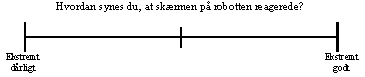
\includegraphics[width =\textwidth]{Figure/TilpasningAfSkalaer/TilpassetSkaermensReaktion} 
\caption{Tilpasset skala til: \textit{Hvordan synes du skærmen på robotten reagerede?}.}
\label{fig:TilpasningSkaermensReaktion}
\end{figure}
\noindent
%
%
\begin{figure}[H]
\centering
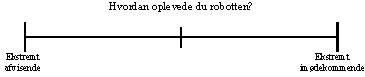
\includegraphics[width =\textwidth]{Figure/TilpasningAfSkalaer/TilpassetOplevede} 
\caption{Tilpasset skala til: \textit{Hvordan oplevede du robotten?}.}
\label{fig:TilpasningOplevede}
\end{figure}
\noindent
%
%
\begin{figure}[H]
\centering
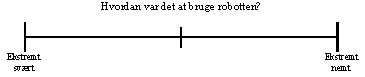
\includegraphics[width =\textwidth]{Figure/TilpasningAfSkalaer/TilpassetHvordanVarDetAtBrugeR} 
\caption{Tilpasset skala til: \textit{Hvordan var det at bruge robotten?}.}
\label{fig:TilpasningBrugAfR}
\end{figure}
\noindent
%
%
\begin{figure}[H]
\centering
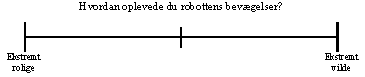
\includegraphics[width =\textwidth]{Figure/TilpasningAfSkalaer/TilpassetBevaegelserR} 
\caption{Tilpasset skala til: \textit{Hvordan oplevede du robottens bevægelser?}.}
\label{fig:TilpasningBevaegelserR}
\end{figure}
\noindent
%
DE TRE FØLGENDE SKALAER HØRER TIL DEN SAMME GRUPPE OG SKAL PRÆSENTERES PÅ DEN SAMME SKÆRM.
%
\begin{figure}[H]
\centering
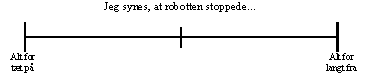
\includegraphics[width =\textwidth]{Figure/TilpasningAfSkalaer/TilpassetRStoppede} 
\caption{Tilpasset skala til: \textit{Jeg synes at robotten stoppede...}.}
\label{fig:TilpasningRStoppede}
\end{figure}
\noindent
%

%
\begin{figure}[H]
\centering
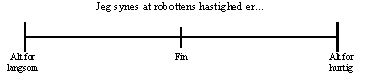
\includegraphics[width =\textwidth]{Figure/TilpasningAfSkalaer/TilpassetHastighedR} 
\caption{Tilpasset skala til: \textit{Jeg synes at robottens hastighed er...}.}
\label{fig:TilpasningHastighedR}
\end{figure}
\noindent
%
%
\begin{figure}[H]
\centering
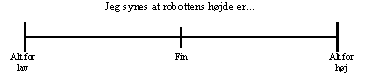
\includegraphics[width =\textwidth]{Figure/TilpasningAfSkalaer/TilpassetHoejdeR} 
\caption{Tilpasset skala til: \textit{Jeg synes at robottens højde er...}.}
\label{fig:TilpasningHoejdeR}
\end{figure}
\noindent
%
DE SEKS FØLGENDE SKALAER HØRER TIL DEN SAMME GRUPPE OG SKAL PRÆSENTERES PÅ DEN SAMME SKÆRM.
%
\begin{figure}[H]
\centering
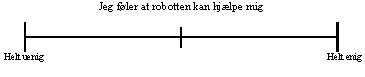
\includegraphics[width =\textwidth]{Figure/TilpasningAfSkalaer/TilpassetRobottenKanHjaelpe} 
\caption{Tilpasset skala til: \textit{Jeg føler at robotten kan hjælpe mig}.}
\label{fig:TilpasningRobottenKanHjaelpe}
\end{figure}
\noindent
% 
%
\begin{figure}[H]
\centering
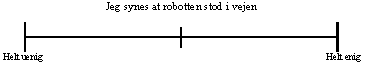
\includegraphics[width =\textwidth]{Figure/TilpasningAfSkalaer/TilpassetRobottenErIVejen} 
\caption{Tilpasset skala til: \textit{Jeg synes at robotten er i vejen}.}
\label{fig:TilpasningRobottenErIVejen}
\end{figure}
\noindent
% 
%
\begin{figure}[H]
\centering
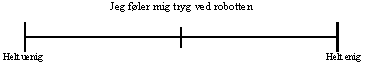
\includegraphics[width =\textwidth]{Figure/TilpasningAfSkalaer/TilpassetTrygVedR} 
\caption{Tilpasset skala til: \textit{Jeg føler mig tryg ved robotten}.}
\label{fig:TilpasningTrygVedR}
\end{figure}
\noindent
% 
%
\begin{figure}[H]
\centering
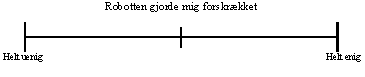
\includegraphics[width =\textwidth]{Figure/TilpasningAfSkalaer/TilpassetForskraekket} 
\caption{Tilpasset skala til: \textit{Robotten gjorde mig forskrækket}.}
\label{fig:TilpasningForskraekket}
\end{figure}
\noindent
% 
%
\begin{figure}[H]
\centering
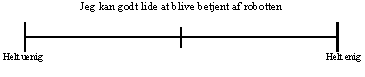
\includegraphics[width =\textwidth]{Figure/TilpasningAfSkalaer/TilpassetLideBetjening} 
\caption{Tilpasset skala til: \textit{Jeg kan godt lide at blive betjent af robotten}.}
\label{fig:TilpasningLideBetjening}
\end{figure}
\noindent
% 
%
\begin{figure}[H]
\centering
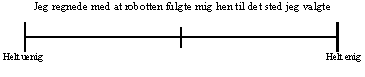
\includegraphics[width =\textwidth]{Figure/TilpasningAfSkalaer/TilpassetRobottenFulgteMigDetRigtigeStedHen} 
\caption{Tilpasset skala til: \textit{Jeg regnede med at robotten fulgte mig hen til det sted jeg valgte}.}
\label{fig:TilpasningRobottenFulgte}
\end{figure}
\noindent
%
DE TO FØLGENDE SKALAER HØRER TIL DEN SAMME GRUPPE OG SKAL PRÆSENTERES PÅ DEN SAMME SKÆRM.
%
\begin{figure}[H]
\centering
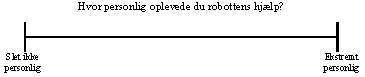
\includegraphics[width =\textwidth]{Figure/TilpasningAfSkalaer/TilpassetPersonligHjaelp} 
\caption{Tilpasset skala til: \textit{Hvor personlig oplevede du robottens hjælp?}.}
\label{fig:TilpasningPersonligHjaelp}
\end{figure}
\noindent
%
%
\begin{figure}[H]
\centering
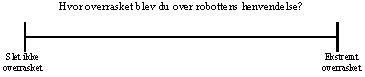
\includegraphics[width =\textwidth]{Figure/TilpasningAfSkalaer/TilpassetOverrasketOverR} 
\caption{Tilpasset skala til: \textit{Hvor overrasket blev du over robottens henvendelse?}.}
\label{fig:TilpasningOverrasketOverR}
\end{figure}
\noindent
%  
DE FØLGENDE SKALA ER ALLE SAT OP PÅ SAMME MÅDE  
%
\begin{figure}[H]
\centering
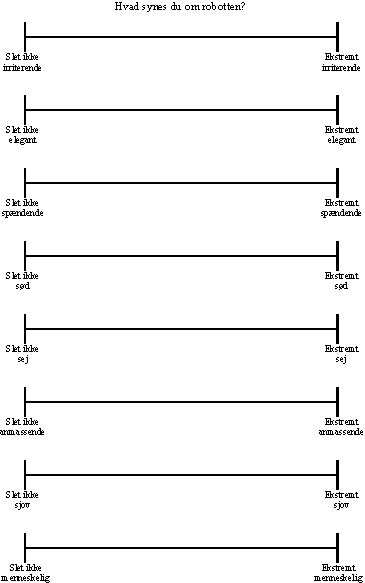
\includegraphics[width =\textwidth]{Figure/TilpasningAfSkalaer/HvadSynesDuOmR} 
\caption{Tilpasset skalaer til: \textit{Hvad synes du om robotten}.}
\label{fig:TilpasningHvadSynesDuOmR}
\end{figure}
\noindent
%
 
